\documentclass[12pt]{article}
\usepackage{geometry}
\geometry{a4paper, margin=1in}
\usepackage{graphicx}
\usepackage{titlesec}
\usepackage{xcolor}
\usepackage{hyperref}
\usepackage{fancyhdr}
\usepackage{enumitem}

% Formatting
\titleformat{\section}{\large\bfseries}{\thesection.}{0.5em}{}
\pagestyle{fancy}
\setlength{\headheight}{15pt}
\fancyhf{}
\rhead{EE175A/B - Weekly Progress Report}
\lhead{Battery Management and Communication System}
\rfoot{Page \thepage}

\begin{document}

\begin{center}
    {\Large \textbf{Weekly Progress Report (WPR)}} \\[6pt]
    {\large \textbf{Battery Management and Communication System (BMS)}} \\[2pt]
    \rule{0.8\textwidth}{0.5pt} \\[6pt]
\end{center}

\noindent
\textbf{Team:} Kaushik Vada, Christian Kim, Connor Stewart, Nick Poon \\[3pt]
\textbf{Course:} EE175B - Senior Design II \\
\textbf{Instructor:} Prof. Roman Chomko \\
\textbf{Week:}(\textit{Feb 16 - Feb 22, 2026}) \\[8pt]

\vspace{1em}

\section{Work Completed This Week}
\begin{itemize}[leftmargin=1cm]
    \item Implemented TIM4-based PWM fan control on the STM32F303RC (PB6, 1\,kHz PWM, 0--100\% duty cycle) by integrating the HAL TIM and TIM-extended driver libraries into the firmware project.
    \item Designed a temperature-driven automatic fan speed curve with five operating points (30\,°C $\rightarrow$ 20\%, 35\,°C $\rightarrow$ 35\%, 40\,°C $\rightarrow$ 55\%, 45\,°C $\rightarrow$ 75\%, 50\,°C $\rightarrow$ 100\%) with linear interpolation between breakpoints.
    \item Added 2\,°C hysteresis to the auto fan control loop to prevent rapid duty-cycle oscillation around a threshold temperature.
    \item Implemented manual fan override mode (\texttt{Fan\_SetManualDuty} / \texttt{Fan\_SetAutoMode}) controllable via USB serial commands from the desktop GUI.
    \item Integrated 10-channel STM32 ADC thermistor reading using the Beta-model NTC equation (Beta = 3950, $R_0$ = 10\,k$\Omega$) to convert raw ADC values to degrees Celsius.
    \item Added BQ76930 pack current sensing via a 20\,m$\Omega$ shunt resistor (0.422\,mA per LSB), including auto-detection of I2C device address (0x08 or 0x18) and CRC mode.
    \item Extended the serial data stream parser to support multi-format fan telemetry: combined inline (\texttt{FAN:AUTO=1,DUTY=55,RPM=1485}), separate RPM (\texttt{Fan -> 783 RPM}), and status line (\texttt{fan\_auto:1 fan\_duty:29}) formats.
    \item Added indexed cell voltage and temperature token parsing (\texttt{C1:3.54 C2:3.56\,\ldots} and \texttt{T1:25.0 T2:24.5\,\ldots}) to correctly reconstruct multi-cell frames from per-cell serial tokens.
    \item Improved multi-line frame assembly in the serial parser with timeout-based frame finalization and persistent last-known fan control data propagation across frame boundaries.
    \item Added a JS command queue polling mechanism (50\,ms interval) in the GUI launcher as a fallback for the QWebChannel \texttt{sendCommand} path to improve firmware command reliability.
    \item Implemented iCloud path detection and Qt runtime bootstrapping on macOS to resolve plugin loading failures from iCloud Drive-backed virtual environments.
\end{itemize}

\vspace{1em}

\section{Challenges Encountered}
\begin{itemize}[leftmargin=1cm]
    \item Integrating the STM32 HAL TIM driver required manually adding \texttt{stm32f3xx\_hal\_tim.c} and \texttt{stm32f3xx\_hal\_tim\_ex.c} to the project, as they were not included in the initial CubeMX-generated build, causing linker failures until resolved.
    \item Selecting an appropriate PWM frequency and duty resolution involved balancing audible fan noise (too low a frequency causes buzzing) against timer counter overflow constraints at 48\,MHz.
    \item The ADC NTC thermistor readings required slow sampling time (\texttt{ADC\_SAMPLETIME\_601CYCLES\_5}) to stabilize on the high-impedance thermistor network; faster settings produced inconsistent raw values.
    \item The serial parser needed to handle mixed structured and unstructured lines without incorrectly discarding indexed-token telemetry frames that arrive interleaved with human-readable status text.
\end{itemize}

\vspace{1em}

\section{Work Plan for Next Week}
\begin{itemize}[leftmargin=1cm]
    \item Connect BMS hardware and validate a live end-to-end data stream from the STM32 firmware through USB to the desktop GUI, including cell voltages, temperatures, current, and fan telemetry.
    \item Calibrate NTC thermistor readings against a reference thermometer and tune the Beta coefficient if needed.
    \item Test the closed-loop fan control with real thermistor data and validate auto/manual switching via GUI commands.
    \item Begin implementing Fault Management System (FMS) logic on the firmware side and integrate fault status alerts into the GUI dashboard.
\end{itemize}

\vspace{1em}

\section{Appendix A - System Block Diagram}
\begin{center}
    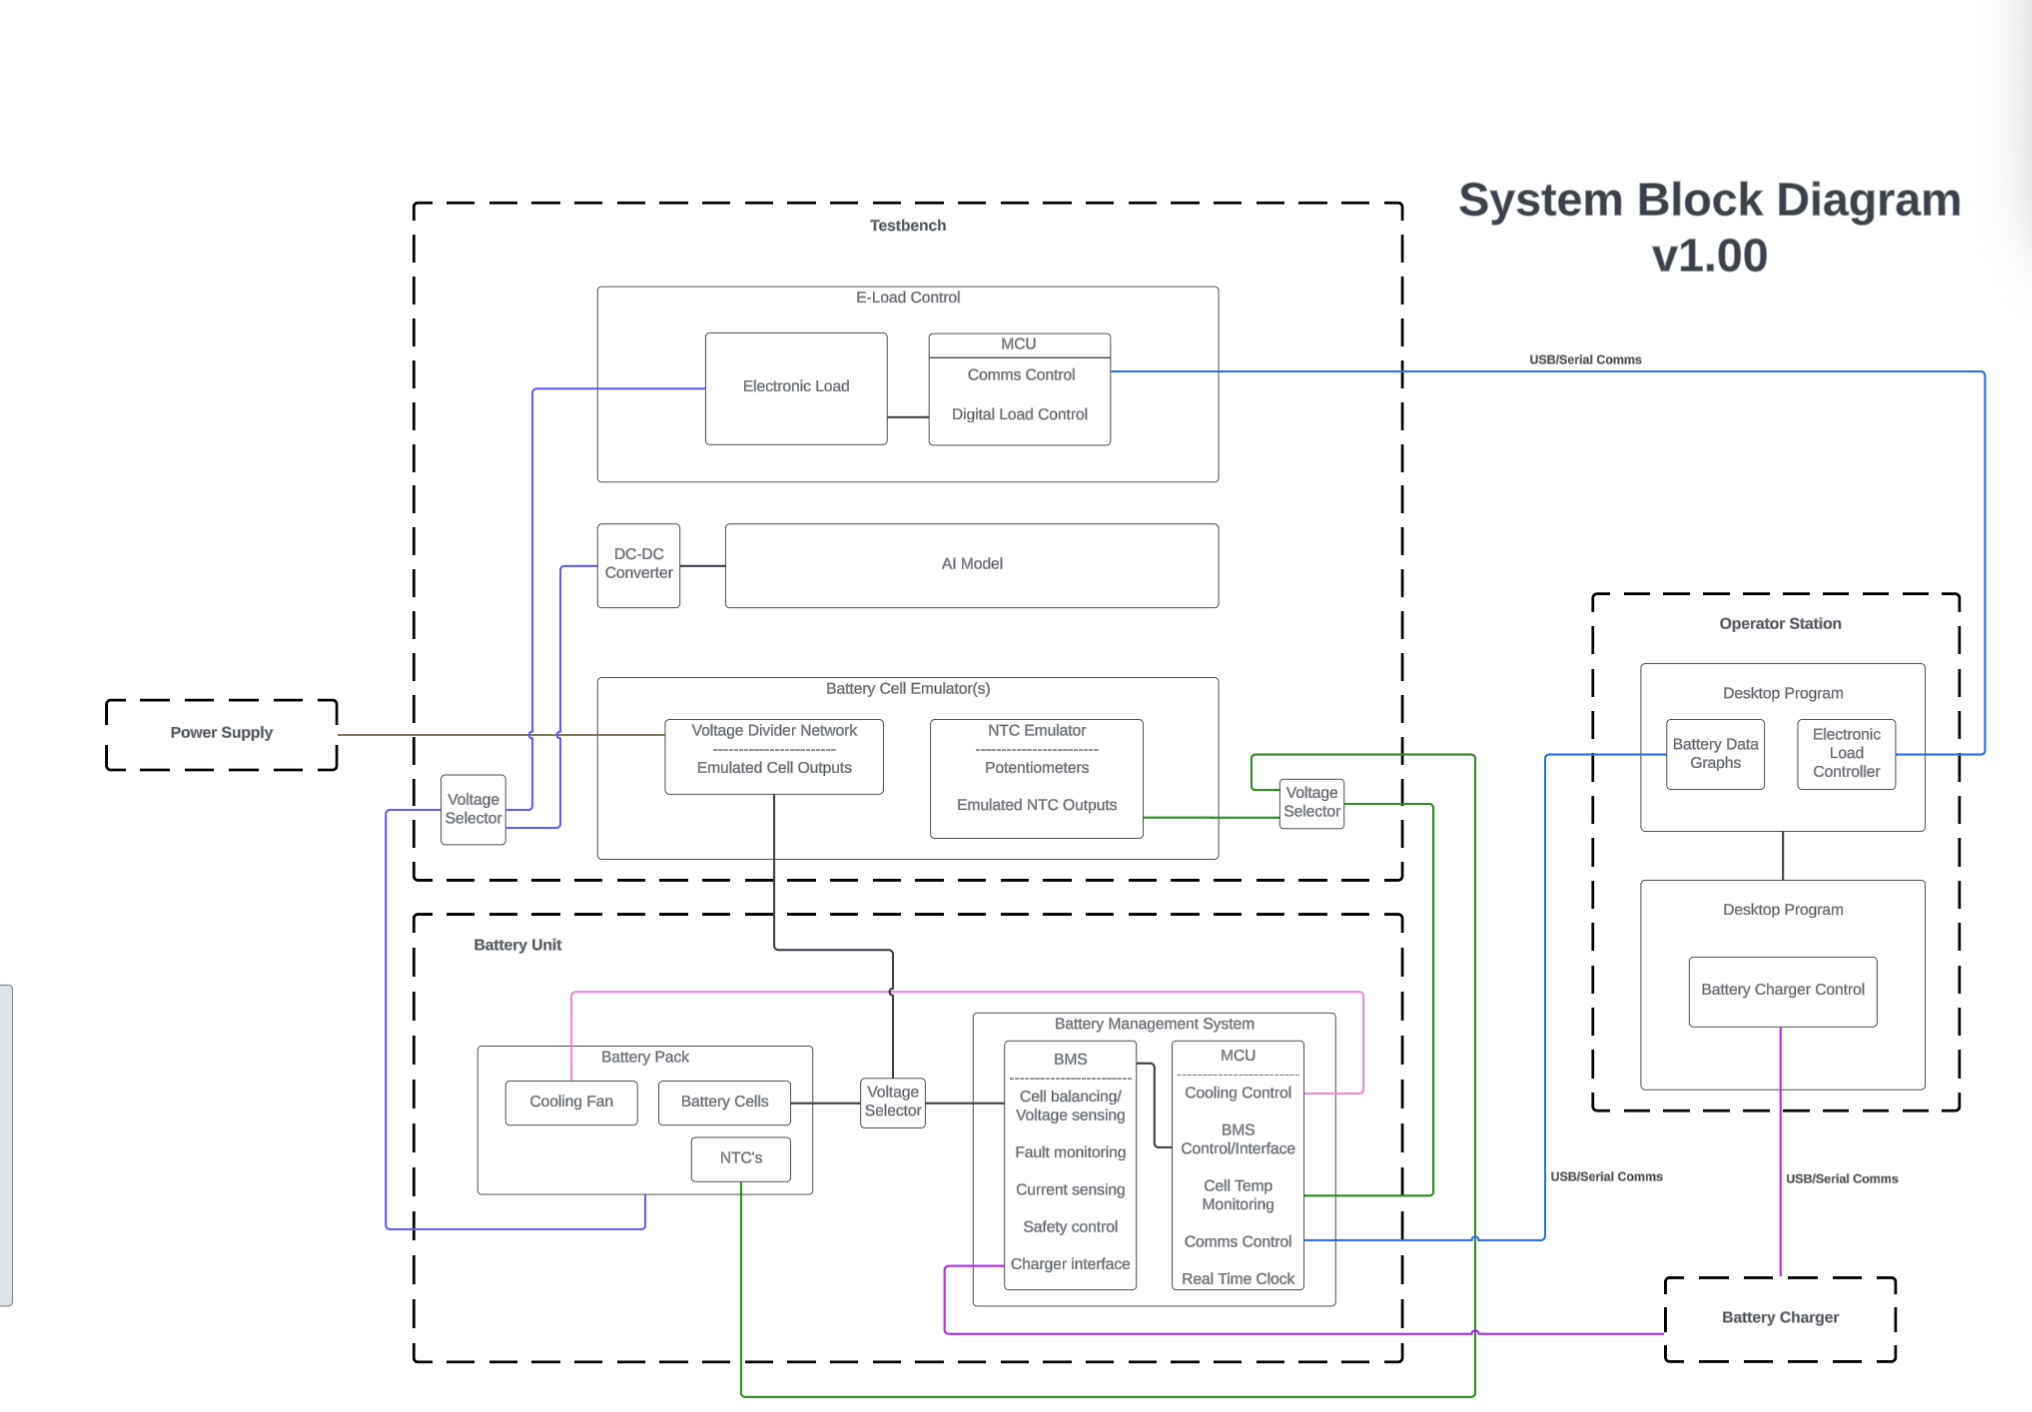
\includegraphics[width=0.95\textwidth]{bms_block_diagram.png} [Figure 1]
\end{center}
\noindent
\textit{Figure A1:} Updated System Block Diagram showing battery domain, isolation components, STM32 communication, and host interface (Source: EE175 Project Report).

\vspace{1em}

\section{Appendix B - Enclosure Visualization}
\begin{center}
    \includegraphics[width=0.95\textwidth]{BMS_enclosure.png} [Figure 2]
\end{center}
\noindent
\textit{Figure B1:} 3D rendering of BMS enclosure with semi-transparent lid, showing airflow, fan, USB-C port, and internal component placement.

\vspace{1em}

\section{Appendix C - Battery Pack Implementation}
\begin{center}
    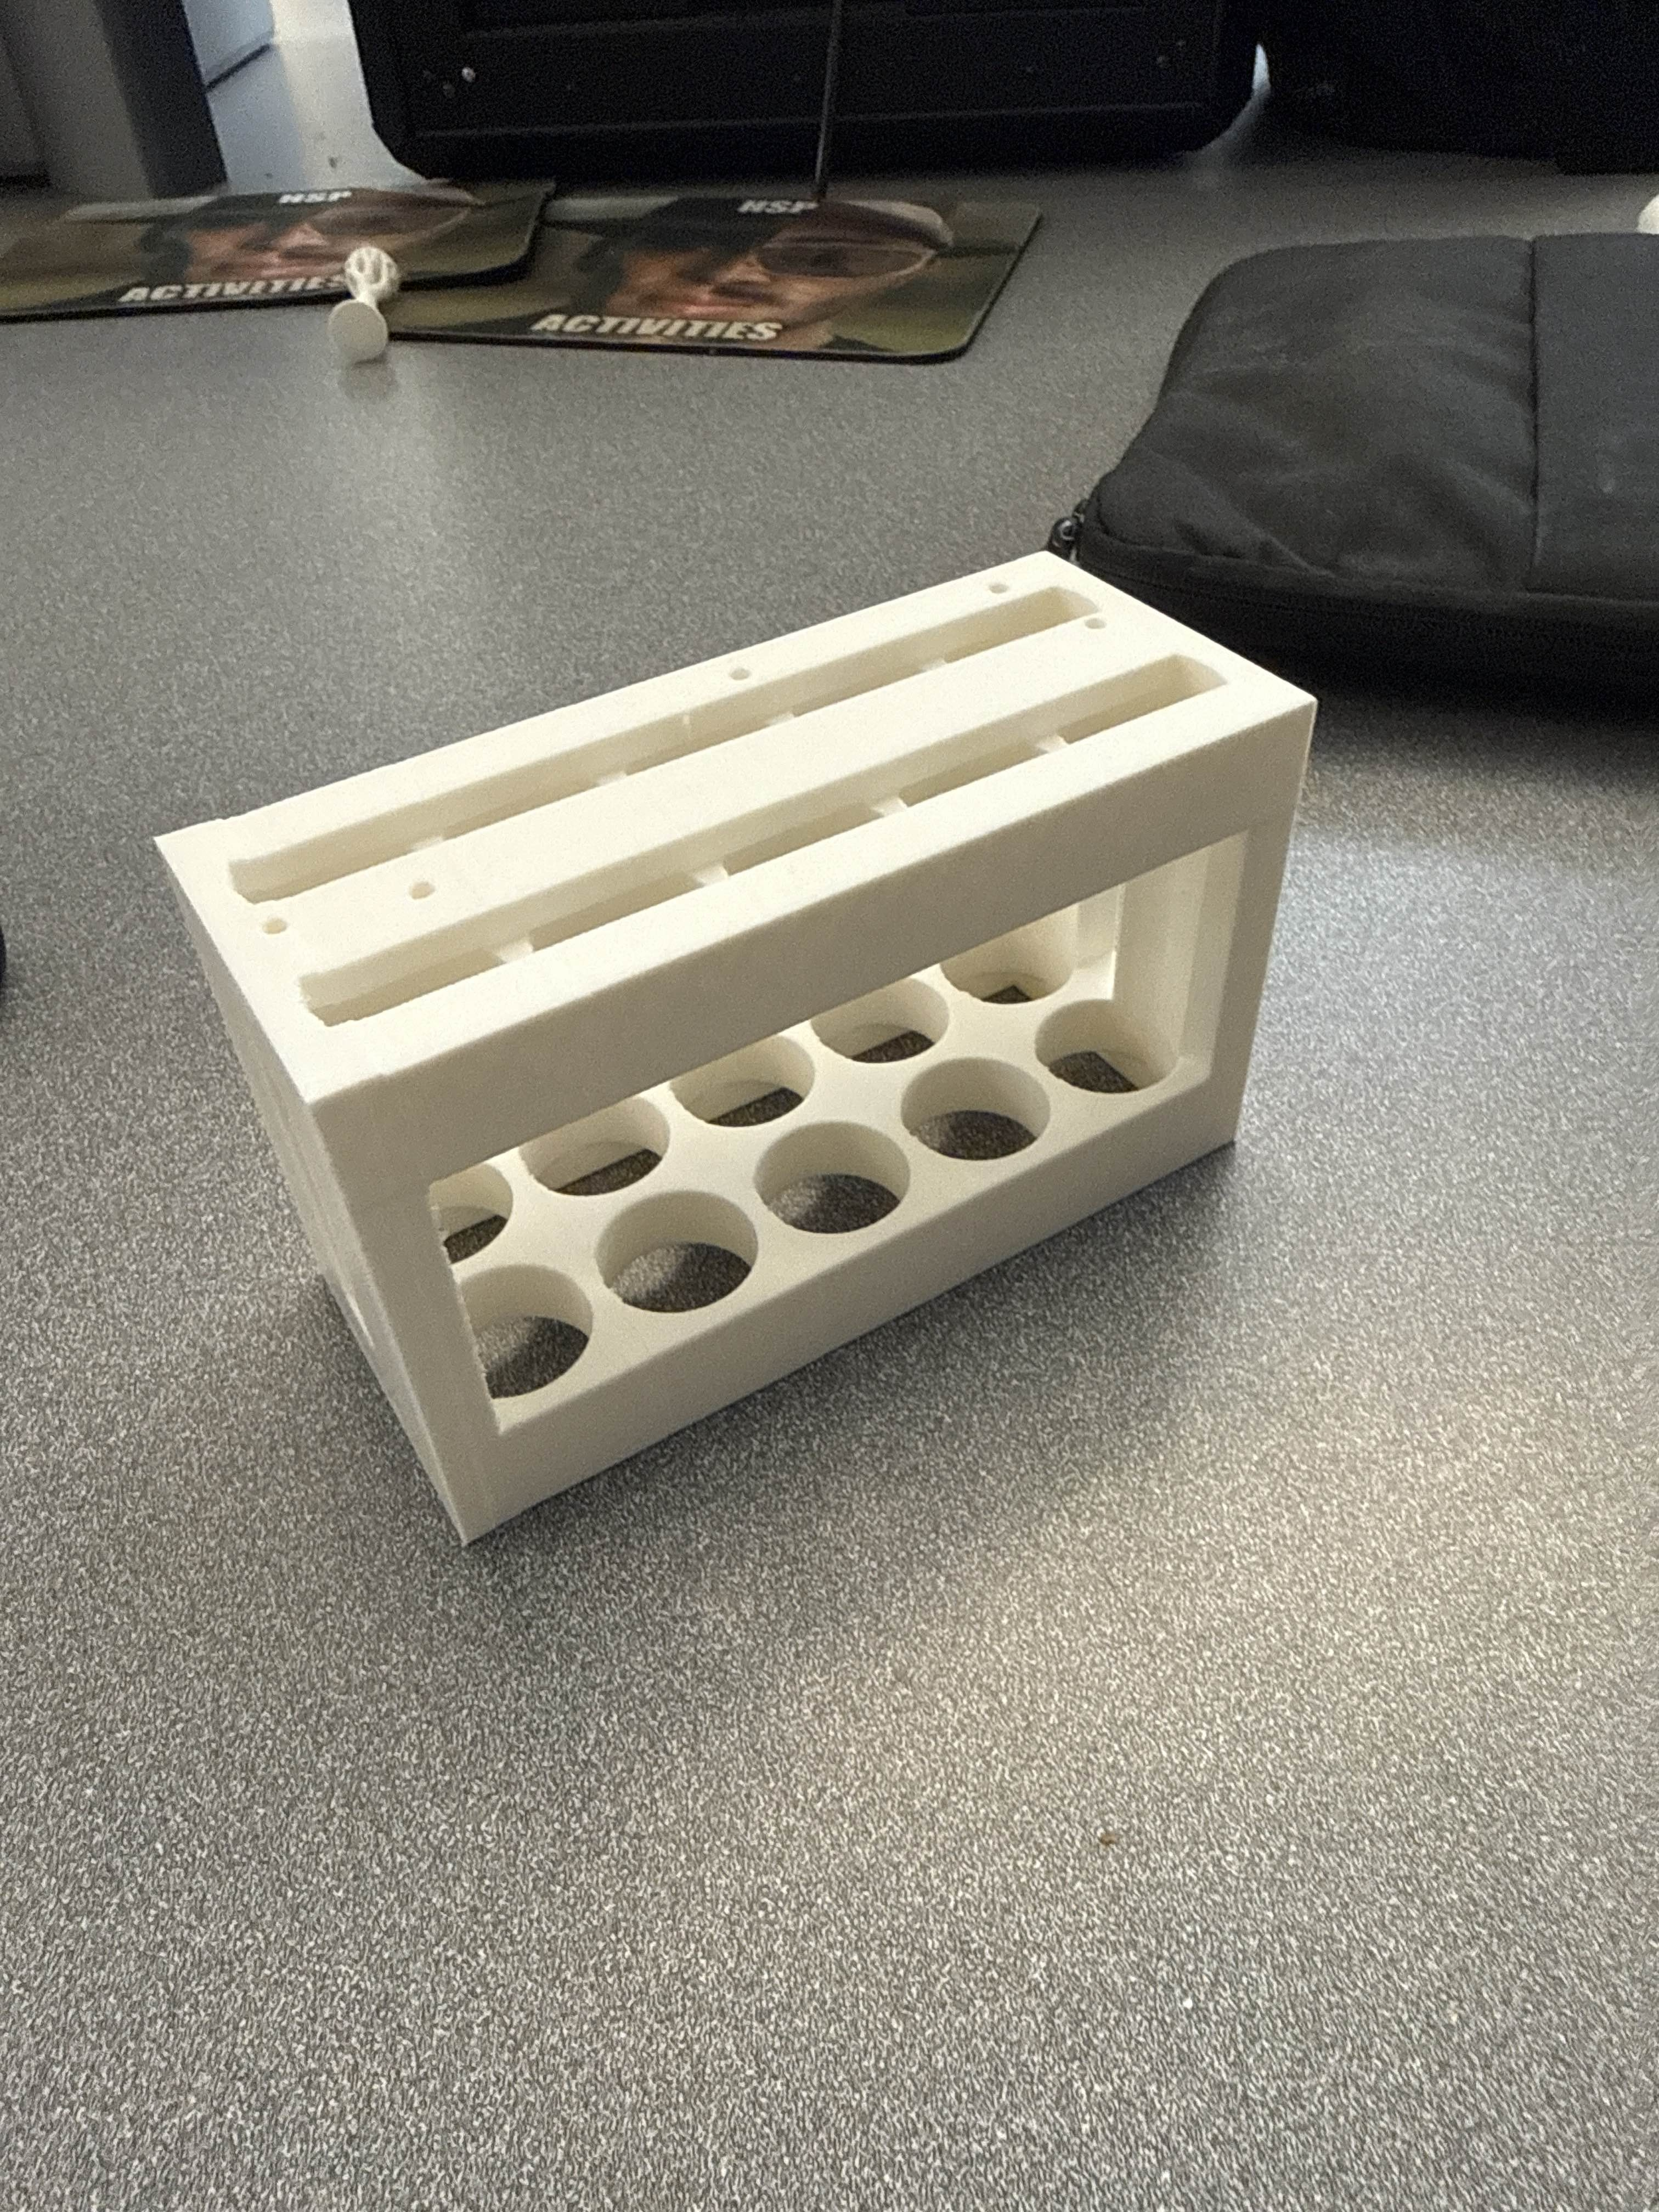
\includegraphics[width=0.95\textwidth]{Battery_Pack.png} [Figure 3]
\end{center}
\noindent
\textit{Figure C1:} Battery pack assembly showing cell arrangement and integration with the BMS unit.

\vspace{1em}

\section{Appendix D - BMS GUI Visualization}
\begin{center}
    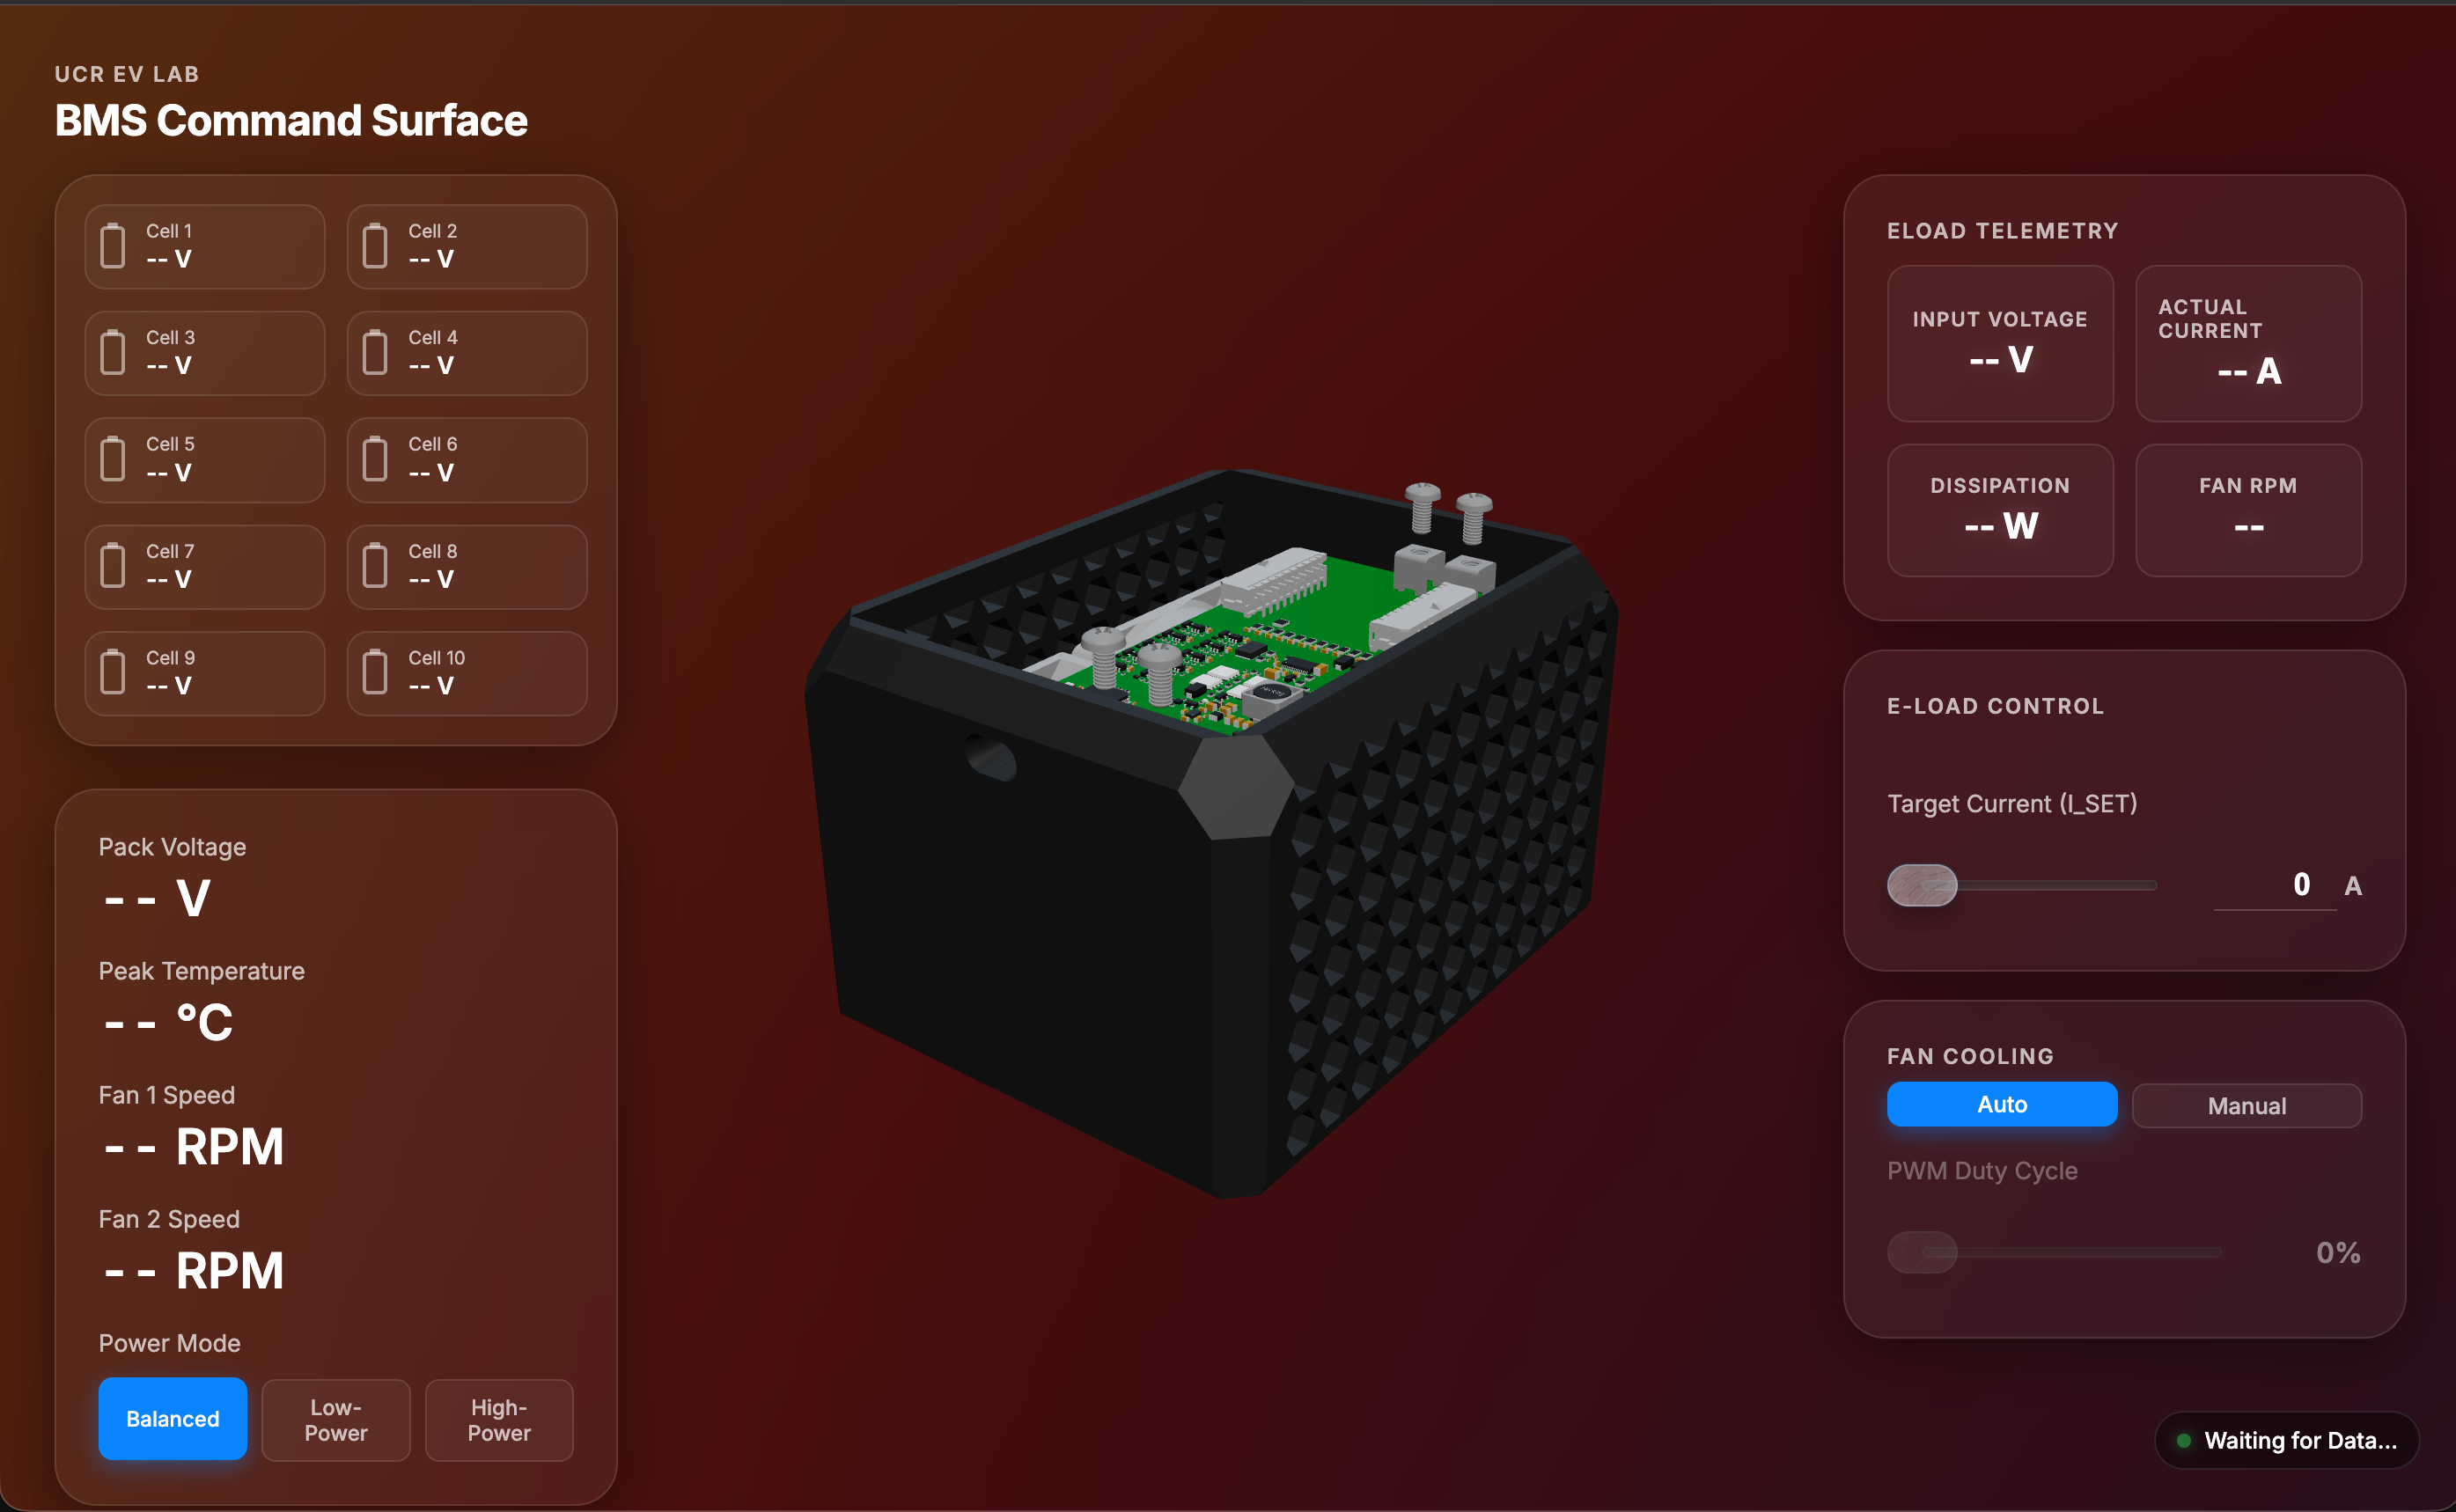
\includegraphics[width=0.95\textwidth]{BMS_GUI.png} [Figure 4]
\end{center}
\noindent
\textit{Figure D1:} Screenshot of the custom Python GUI displaying real-time BMS data, including individual cell voltages, pack voltage, current, and temperature readings.

\vspace{1em}

\section{Appendix E - Firmware Development}
\begin{center}
    
\includegraphics[width=0.95\textwidth]{firmware.png} [Figure 5]
\end{center}
\noindent
\textit{Figure E1:} USB-Connection-Firmware project in STM32CubeIDE showing HAL driver integration and peripheral initialization for the STM32F303RC microcontroller, including the newly added TIM4 PWM fan control peripheral.

\end{document}
